% Load the kaobook class
\documentclass[
	fontsize=10pt, % Base font size
	twoside=false, % Use different layouts for even and odd pages (in particular, if twoside=true, the margin column will be always on the outside)
	%open=any, % If twoside=true, uncomment this to force new chapters to start on any page, not only on right (odd) pages
	secnumdepth=1, % How deep to number headings. Defaults to 1 (sections)
]{kaobook}

% Choose the language
\usepackage[english]{babel} % Load characters and hyphenation
\usepackage[english=british]{csquotes}	% English quotes

% Load packages for testing
\usepackage{blindtext}
%\usepackage{showframe} % Uncomment to show boxes around the text area, margin, header and footer
%\usepackage{showlabels} % Uncomment to output the content of \label commands to the document where they are used

% Load the bibliography package
\usepackage{kaobiblio}
\addbibresource{minimal.bib} % Bibliography file

% Load mathematical packages for theorems and related environments
\usepackage{kaotheorems}

% Load the package for hyperreferences
\usepackage{kaorefs}

% epigraphs for chapters
\usepackage{epigraph} 
\renewcommand{\epigraphflush}{flushleft}

% highlighting 
\usepackage{color,soul}

% make backticks, backticks
\usepackage{upquote}


\graphicspath{{img/}{./}} % Paths where images are looked for

\newcommand\kw[1]{\textbf{#1}}

\newenvironment{absolutelynopagebreak}
  {\par\nobreak\vfil\penalty0\vfilneg
   \vtop\bgroup}
  {\par\xdef\tpd{\the\prevdepth}\egroup
   \prevdepth=\tpd}

\newcommand\margingraphic[2]{
  \marginpar{%
    \includegraphics[width=\marginparwidth]{#1}
    \captionof{figure}{#2}
  }
}

\makeindex[columns=3, title=Alphabetical Index, intoc] % Make LaTeX produce the files required to compile the index


\begin{document}

%----------------------------------------------------------------------------------------
%	BOOK INFORMATION
%----------------------------------------------------------------------------------------

% \titlehead{Document Template}
\title{Stackschool}
\author{ACM Hack}
\date{}

%----------------------------------------------------------------------------------------

\frontmatter % Denotes the start of the pre-document content, uses roman numerals

%----------------------------------------------------------------------------------------
%	COPYRIGHT PAGE
%----------------------------------------------------------------------------------------

% \makeatletter
% \uppertitleback{\@titlehead} % Header

% \lowertitleback{
% 	\textbf{Disclaimer} \\
% 	You can edit this page to suit your needs. For instance, here we have a no copyright statement, a colophon and some other information. This page is based on the corresponding page of Ken Arroyo Ohori's thesis, with minimal changes.
	
% 	\medskip
	
% 	\textbf{No copyright} \\
% 	\cczero\ This book is released into the public domain using the CC0 code. To the extent possible under law, I waive all copyright and related or neighbouring rights to this work.
	
% 	To view a copy of the CC0 code, visit: \\\url{http://creativecommons.org/publicdomain/zero/1.0/}
	
% 	\medskip
	
% 	\textbf{Colophon} \\
% 	This document was typeset with the help of \href{https://sourceforge.net/projects/koma-script/}{\KOMAScript} and \href{https://www.latex-project.org/}{\LaTeX} using the \href{https://github.com/fmarotta/kaobook/}{kaobook} class.
	
% 	\medskip
	
% 	\textbf{Publisher} \\
% 	First printed in May 2019 by \@publishers
% }
% \makeatother

%----------------------------------------------------------------------------------------
%	DEDICATION
%----------------------------------------------------------------------------------------

% \dedication{
% 	The harmony of the world is made manifest in Form and Number, and the heart and soul and all the poetry of Natural Philosophy are embodied in the concept of mathematical beauty.\\
% 	\flushright -- D'Arcy Wentworth Thompson
% }

%----------------------------------------------------------------------------------------
%	OUTPUT TITLE PAGE AND PREVIOUS
%----------------------------------------------------------------------------------------

% Note that \maketitle outputs the pages before here
\maketitle

%----------------------------------------------------------------------------------------
%	PREFACE
%----------------------------------------------------------------------------------------

% \chapter*{Preface}

% \blindtext

%----------------------------------------------------------------------------------------
%	TABLE OF CONTENTS & LIST OF FIGURES/TABLES
%----------------------------------------------------------------------------------------

\begingroup % Local scope for the following commands

% Define the style for the TOC, LOF, and LOT
%\setstretch{1} % Uncomment to modify line spacing in the ToC
%\hypersetup{linkcolor=blue} % Uncomment to set the colour of links in the ToC
\setlength{\textheight}{230\vscale} % Manually adjust the height of the ToC pages

% Turn on compatibility mode for the etoc package
\etocstandarddisplaystyle % "toc display" as if etoc was not loaded
\etocstandardlines % "toc lines as if etoc was not loaded

\tableofcontents % Output the table of contents

% \listoffigures % Output the list of figures

% Comment both of the following lines to have the LOF and the LOT on different pages
\let\cleardoublepage\bigskip
\let\clearpage\bigskip

% \listoftables % Output the list of tables

\endgroup

%----------------------------------------------------------------------------------------
%	MAIN BODY
%----------------------------------------------------------------------------------------

\mainmatter % Denotes the start of the main document content, resets page numbering and uses arabic numbers
\setchapterstyle{kao} % Choose the default chapter heading style

\setchapterpreamble[u]{\margintoc}

\chapter{Introduction to Full Stack}

\epigraph{\emph{"There are two mistakes one can make along the road to truth: not going all the way, and not starting."}}{ -- Alan Cohen}

As a beginner, full stack development can be quite intimidating. Looking it up yields a seemingly endless list of languages and technologies that you must learn in order to even get started, and who has time for that? The good news is that we can drastically limit the number of things to learn by making a couple of strategic decisions before we start. The bad news is that you will still have to learn about six technologies, three of which we're going to assume you have at least a basic understanding of going into the workshop series. That being said, stick with us! By the end of this, you'll have no trouble making your own full stack application to rival Facebook or Twitter and you'll have a lot of fun doing it. 

Before we get into any actual content, allow me to first give you some advice on approaching this series\sidenote{And I guess learning in general.}. At first, it's not going to be easy. It'll be frustrating and you'll bang your head against the wall and you'll want to quit. You'll want to quit often. But don't. Stick with it, and eventually you'll make progress. You'll figure out what was causing that unreadable error or that 400 response code, and the feeling of accomplishment will be like no other. Little victories will begin to pile up around you and, before you know it, you'll have a completed full stack app ready to show off to the world. It won't be easy, but nothing worth doing ever is. And keep in mind you're not on your own here! You have a team of twenty passionate, wonderful Hack officers ready to help you through your struggles. All you need to do is reach out!\sidenote{Which you can do in person or on \href{https://discord.gg/T5Nu5hTs7s}{discord}!}

Another piece of advice on learning: it's often helpful to start with an understanding of surface level concepts and dig deeper once you have those mastered.\sidenote{Keep in mind there are many different kinds of learners, so what works for one person may not work for another and vice versa. This is just a suggestion!} This is the approach we will mostly take in this workshop series. Our weekly workshops will provide a high level view of things in order to get you started, offering occasional nuggets of deeper insight, while the textbook will usually be the place to go if you want a deeper understanding. I highly recommmend utilizing both if you truly want to learn the material. If you would prefer, you can also skim the textbook ahead of our workshops and get an idea of the content that way. Whatever works best for you! Throughout the series, we'll show the entire process of building a simple full stack app. By the end, hopefully you'll be able to make your own!

\section{Prerequisites}

As mentioned, due to time constraints we unfortunately won't be able to cover absolutely \emph{everything} you need in order to make a full stack app. In particular, we'll be assuming a basic understanding of frontend concepts. This includes:

\begin{itemize}
    \item Fundamental Coding Concepts (Think CS31)
    \item Basic Shell Commands (\texttt{cd}, \texttt{ls}, etc. )
    \item HTML/CSS
    \item Javascript
    \item React
\end{itemize}

Luckily, we had an entire workshop series\sidenote{Check out our workshops archive \href{https://hack.uclaacm.com/archive}{here}.} covering these ideas last quarter if you need to catch up! We cover these concepts every year in Hackschool, so check out those workshop recordings/slides/README's before attending. We will be giving slight refreshers on these concepts here, but they'll be very quick and likely difficult to follow if you've never seen them before. Alright, with that out of the way... let's get to the content!

\section{Why Full Stack?}

As any good student should, you may be wondering: \emph{What's the point?} To illustrate that, let's take a look at a website that you're probably familiar with. 

\begin{figure*}[h!]
	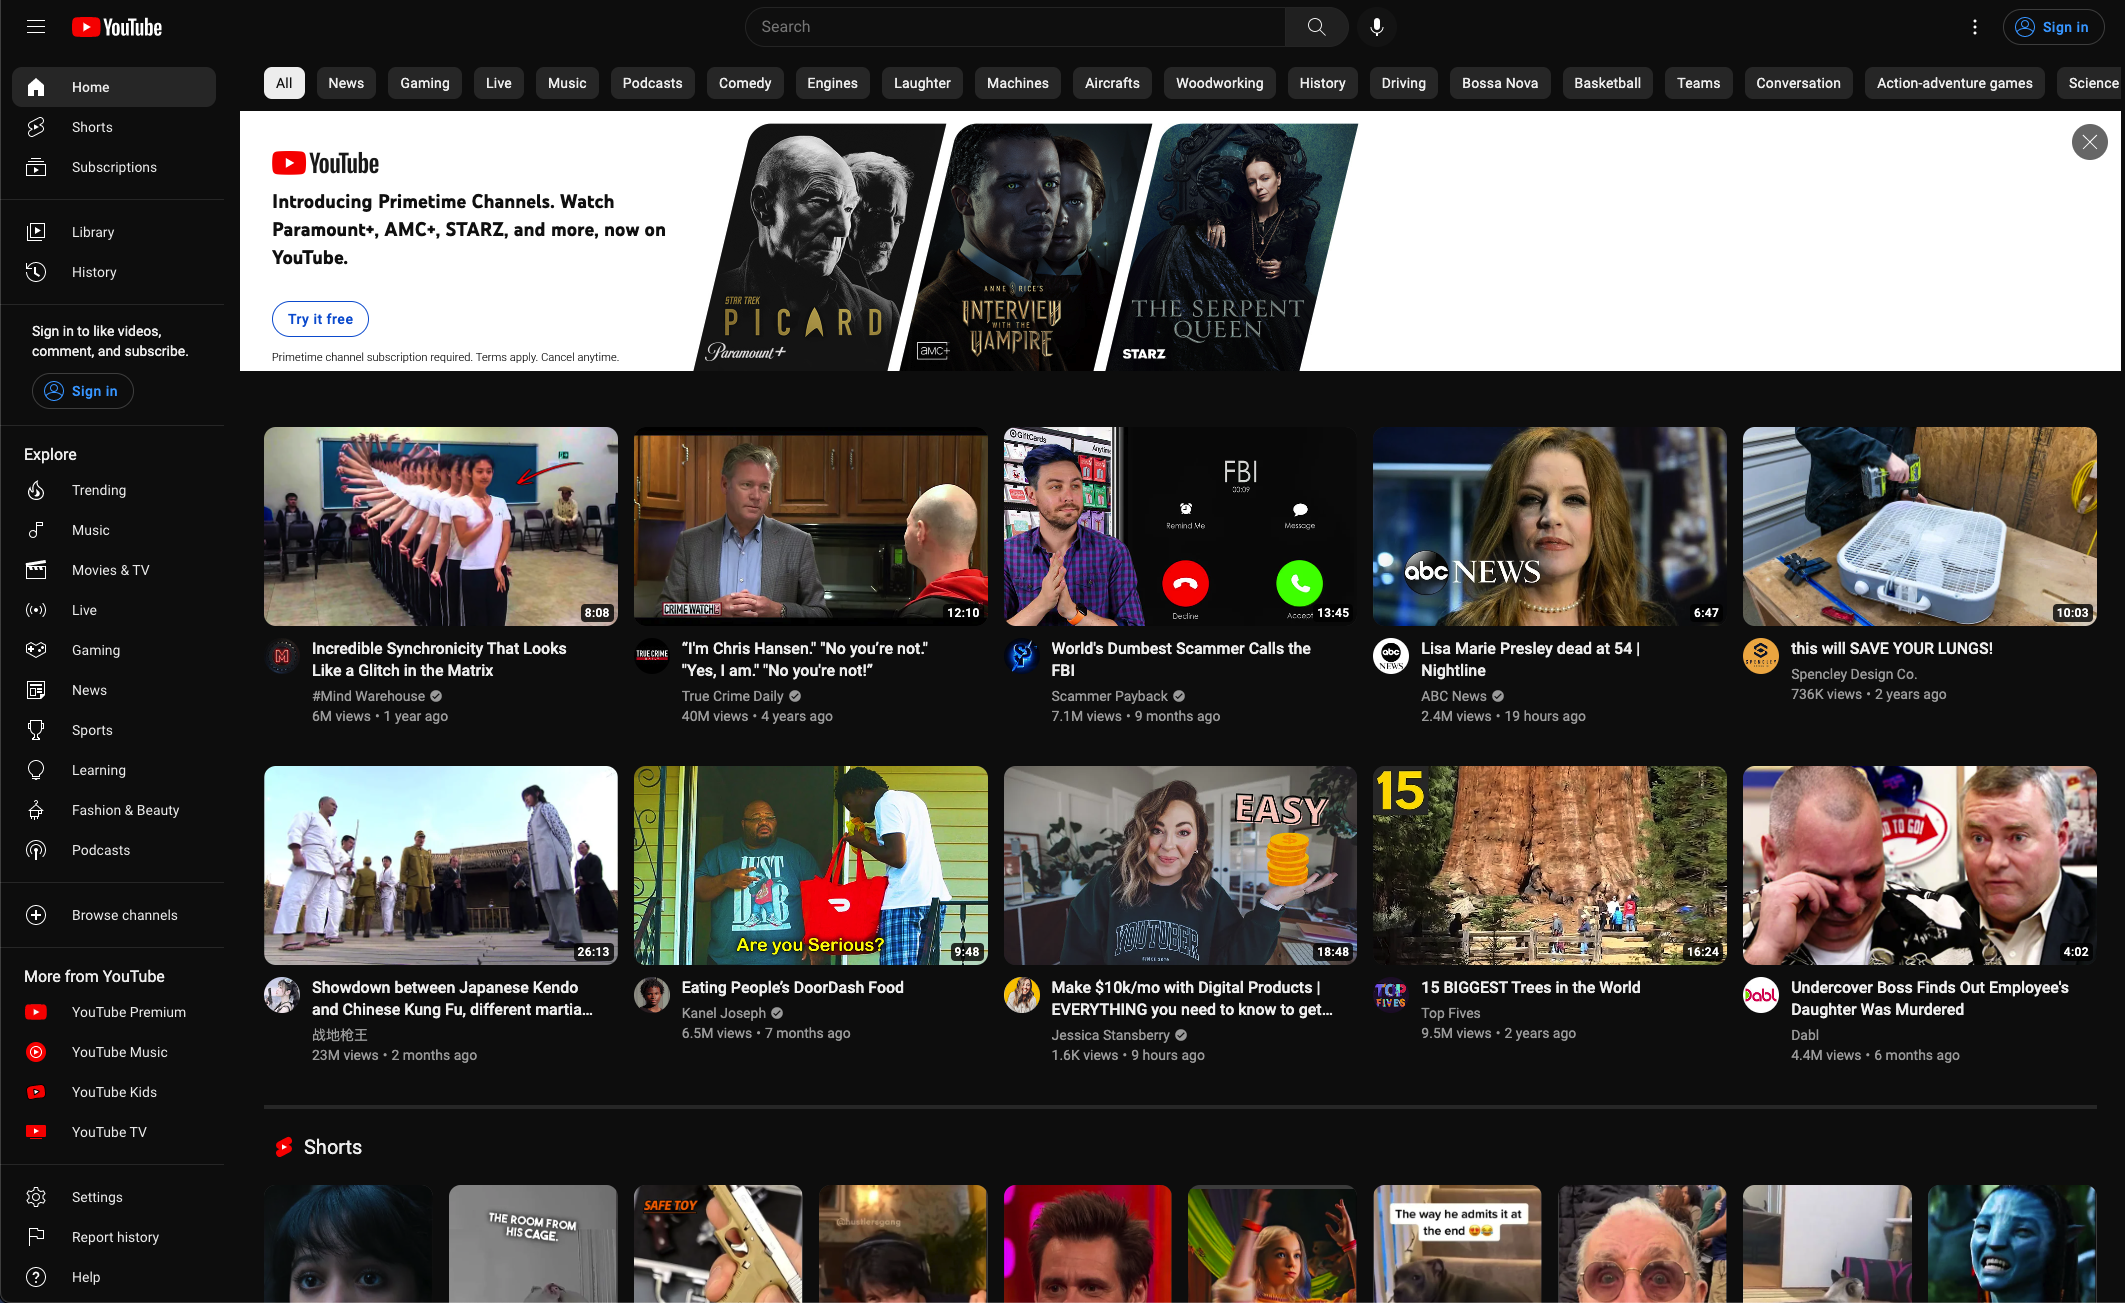
\includegraphics{youtube.png}
    \caption[YouTube]{A screenshot from YouTube's home page. }
\end{figure*}

If we had to design YouTube from scratch, how might we do it? The most obvious component is the UI. It's likely that some mix of HTML/CSS is used in order to deliver the experience you see in the screenshot. There are several other things to think about, however. For instance, where do the videos come from? They're clearly not all hardcoded into the website as that would be a nightmare to maintain. You'll also notice that when you refresh the page, YouTube will adjust which videos it recommends to you to ensure it never gets stale. It takes things a step further if you sign in, tailoring its recommendations based on your previous viewing history. How are they doing this? 

Unfortunately, making a website as intricate as YouTube is impossible without incorporating the full stack. In order to store all the videos and users, something called a \kw{database} is used. Recommendations are determined by an algorithm on a \kw{server} and communicated to the \kw{client} via an \kw{API}. We'll go over exactly what all of these terms mean, but for now just know that they are each essential components of a full stack application. Each of these components works together in order to deliver a product that millions of people use everyday! And it's not just YouTube. The vast majority of websites and apps you frequent\sidenote{Google, Instagram, Twitter, Facebook, BeReal. All of these are full stack applications!} utilize all of these components in order to give you the best experience possible.

Note that not all websites require the full stack. These websites are known as \kw{static sites}, due to the fact that their content is the same for every user that visits and will not change unless the website itself is updated. One example of such a site is \href{https://hack.uclaacm.com/}{Hack's website}!

\section{What is Full Stack?}

Fullstack refers to all of the technologies that are needed to complete a project. Typically, we consider full stack development to be composed of two main components called the \kw{frontend} and \kw{backend}. Naturally, this begs the question: what's the difference?

\subsection*{Frontend}

Frontend is essentially everything that the user interacts with. Think of everything that you see when you interact with a website: a text box, the colors, buttons, links, navigation bars, pages, etc. Typically, the front end is coded in HTML, CSS, and JavaScript. For our demo, we will be using React.js, which is a JavaScript library that helps us with creating our frontend. Essentially, React provides us with lots of useful library functions and integrations that abstract away many of the tedious parts of web development.\sidenote{Such as DOM interactions. Gross.} 

\subsection*{Backend}

If we look at full stack development as an iceberg\sidenote{Which for some reason is a popular comparison.}, the frontend can be considered its tip. What remains deep underwater is the backend. In contrast to frontend development, backend is essentially everything that the user \kw{does not} see. For questions like "\emph{where does the data that I put into my text box go?}" or "\emph{how does my website authenticate me as a proper user?}", we turn to the backend. The backend is made up of multiple parts as well. The ones that we will be focusing on are the server and the database. In order to introduce you to these technologies, let's take a look at them from a very high level.

\subsubsection*{What's a server?}

A server is essentially a computer or program that serves as the \emph{brains} of your application. It handles everything that our app needs in order to function, such as interacting with our database, computationally intensive tasks, user authentication, and more. There are many technologies available for servers, but here we will discuss a technology called Node in conjunction with a library called Express.  It's here that we define our backend API, which is the interface between our frontend and backend. Servers can also be referred to as backend applications.

\subsubsection*{What's a database?}

A database is just an organized collection of data. It abstracts away the storage and retrieval of data in order to make our lives as full stack developers easier. There are several design philosophies surrounding databases, but two of the most popular are relational and non-relational (also known as NoSQL) databases. We'll briefly cover relational databases here with an emphasis placed on the non-relational side.

This was all super high level, but don't worry! We'll be going over each of these in much more detail in chapters to come.

\section{MERN}

For our workshop series, we will be using the M.E.R.N. stack. Each of these letters stand for a specific technology.
\begin{itemize}
    \item MongoDB: A NoSQL database that stores all of our persistent data that the app needs to function, such as users and posts. 
    \item Express: A backend web application framework. 
    \item React.js: A frontend JavaScript library that will help us create our frontend through several useful abstractions. 
    \item Node.js A Javscript runtime environemnt used for creating servers.
\end{itemize}

\subsection*{Downloads}

Before getting started, make sure you set up the required technologies!

\begin{itemize}
    \item Download and install a text editor: \href{https://code.visualstudio.com/download}{VS Code}
    \item Download and install Node.js: \href{https://nodejs.org/en/download/package-manager/}{Node.js}
    \item Download and install Yarn (our package manager of choice): Run the following command after installing Node: \texttt{npm install --global yarn}\sidenote{Or use corepack.}
    \item Create a MongoDB account: \href{https://www.mongodb.com/}{MongoDB}
\end{itemize}

You're now ready to get started!

\setchapterpreamble[u]{\margintoc}
\chapter{Servers}
\epigraph{\emph{"Simplicity, carried to an extreme, \\ becomes elegance."}}{ -- Jon Franklin}

Servers are probably one of the most misunderstood concepts for new developers. If you put ten new developers in a room, it's a pretty good bet that they've all \emph{heard} of servers. Maybe they've been exposed to them through pop culture. They've seen movies or read books where the nerdy, basement dwelling side character is approached by the charismatic protagonist to "hack into the mainframe" to stop the evil corporation and save the world.\sidenote{Note that a mainframe is just a special name for a server that is capable of performing a large amount of concurrent operations. Whether or not "hacking" into one will save the world is another question.} Or maybe they've come across the terminology at some point while learning about the fundamentals of programming, with their instructors glossing over it saying, "don't worry about this yet." Whatever the case may be, its likely that a majority of the ten new developers you have confined to a room would not be able to tell you what exactly a server does, or why. Or even more fundamentally, what \emph{is} a server? 

In a way, this lack of understanding almost serves as a hint to what a server is: a blackbox\sidenote{A blackbox is a term for an object that takes some input and transforms it into some desired output, with the user not necessarily knowing the details of how it works.} to process and retrieve information. We see this concept, \kw{abstraction}, fairly frequently in programming and Computer Science. Through abstraction, we make it far simpler for others to interact with our programs. It's a very important concept, and we'll be digging into it in detail throughout this chapter. 

This write-off of servers as blackboxes is great if we just want to use them to get some data. It makes our job much easier! In fact, you interact with servers (indirectly) every single day just by browsing the internet\sidenote{Can you imagine if you had to be familiar with all the intricacies of servers just to watch a YouTube video?}. However, when it comes time to create our own, it's important to have a deeper understanding. And that's what we aim to accomplish here! By first instilling in you an idea of the \emph{fundamental} concept of a server\sidenote{Note that we won't go over all the low level implementation details. That's for your upper division CS classes to cover!}, and later showing one possible implementation (among many), we'll break the blackbox open and expose the ideas within.

\section{Servers In General}

Put simply, a server is a computer like any other. What distingishes a regular old computer and a server is that \kw{servers are given the task of listening and responding to requests}. These tend to be requests for data or to perform some task and in general they come from other computers\sidenote{We will see that it's not always the case that requests originate from other computers. A single computer can be both the server and the client, and you'll see that this is actually very common, particularly during the development process of a full stack application.}. We call these "other" computers \kw{clients}. You can think of the interaction between a server and a client in much the same way as the interaction between a customer at a restaurant and the restaurant's staff. Just as a customer can request a glass of water, new silverware, or a half serving of Tiramisu, a client can request some function to be performed or data to be processed and returned. This brings up an important question: how do the client and server communicate? A customer at a restaurant might use English or Portuguese, but unfortunately computers aren't quite there yet. They must have some standard, agreed upon language in order to do so.

\subsection*{The Language of Requests}

In the context of clients and servers, the "language" that is typically used is \kw{HTTP}, or Hypertext Transfer Protocol\sidenote{Note that there are other protocols that can be used, such as WebRTC, and each have their advantages. For now, let's not get into the weeds too much, but I recommend reading up on protocols if you're interested.}. This protocol makes it easier for servers to parse through a client's request due to the fixed format. Take a look at the following example of a real HTTP request:

\begin{lstlisting}[language=html]
    GET / HTTP/1.1
    Host: www.example.com
    User-Agent: Mozilla/5.0
    Accept: text/html,application/xhtml+xml,application/xml;
            q=0.9,image/avif,image/webp,*/*;q=0.8
    Accept-Language: en-GB,en;q=0.5
    Accept-Encoding: gzip, deflate, br
    Connection: keep-alive
\end{lstlisting}

It may seem strange and hard to read as a human, but it is perfectly formatted for computers. We don't have to worry about the exact formatting as creating these requests is typically automated, but I do want to point out one key detail: the word \texttt{GET}. \texttt{GET} indicates to the server the particular action desired by the client, and it is one of several so called \kw{HTTP request methods}. We'll discuss these in more detail and show several examples, so don't worry if you haven't quite grasped the concept yet. For now, here are a few essential methods to be aware of \sidenote[]{There are methods beyond these. Check out Mozilla's \href{https://developer.mozilla.org/en-US/docs/Web/HTTP/Methods}{article} on the subject if you're interested.}: 

\begin{itemize}
    \item \texttt{GET}: indicates a request for some data
    \item \texttt{POST}: submits data to the server which often results in some side effect or change to the server's state
    \item \texttt{PUT}: submits data to the server in order to update an existing resource
    \item \texttt{DELETE}: removes some resource from the server
\end{itemize}

After receiving a well-formed request, the server will perform the specified action and create a \kw{response} to send back to the client. The format of a response is also standardized by HTTP, and here is an example:

\begin{lstlisting}[language=html]
    HTTP/1.1 200 OK
    Date: Mon, 23 May 2005 22:38:34 GMT
    Content-Type: text/html; charset=UTF-8
    Content-Length: 155
    Last-Modified: Wed, 08 Jan 2003 23:11:55 GMT
    Server: Apache/1.3.3.7 (Unix) (Red-Hat/Linux)
    ETag: "3f80f-1b6-3e1cb03b"
    Accept-Ranges: bytes
    Connection: close

    <html>
    <head>
        <title>An Example Page</title>
    </head>
    <body>
        <p>Hello World, this is a very simple HTML document.</p>
    </body>
    </html>
\end{lstlisting}


The first thing you might notice is that the response seems to have HTML embedded into it. Why might that be? Let's come back to that. Take a look at the first line of the response. As before, it indicates that it is following HTTP, but it also has the number 200 and the word \texttt{OK}. This is known as an \kw{HTTP response code} and it represents the result of the server's attempt to address the client's request. In this case, \texttt{200 OK} indicates that the request was successfully, received, understood, and accepted. There are many response codes but they all fall into the following categories:

\begin{itemize}
    \item \texttt{1XX}: informational; the request was received and is being processed
    \item \texttt{2XX}: successful; the request was successfully, received, understood, and accepted
    \item \texttt{3XX}: redirection; further action needs to be taken in order to complete the request
    \item \texttt{4XX}: client error; the request contains bad syntax or cannot be fulfilled
    \item \texttt{5XX}: server error; the server failed to fulfill an apparently valid request
\end{itemize}

You don't have to memorize these, but you'll find that after working with HTTP requests for a while they'll just come naturally. For example, you might be familiar with the infamous code \texttt{404}, which indicates that a resource was not found. You'll come to recognize other codes just like this one.

\begin{kaobox}[title=About the HTML we saw before\dots]
    What was it doing there? It's known as the \kw{body} of the response, and it's being sent back to the client, in essence, because that's what they asked for. Let's break things down. The client sent a \texttt{GET} request, asking the server to send some data back from a particular location (www.example.com). The data that was sent was this HTML code... Do you see where this is going yet? \\ \\
    We know that HTML is used by browsers in order to render web pages, so our client can now successfully render the web page stored on the server. In essence, the client uses this HTTP request in order to receive the data necessary to render a web page! This process happens billions of times per day, and it is the back bone of the whole internet. The internet is built upon servers which store HTML, CSS, and Javascript and your browser uses HTTP requests to request them to be sent to you! Obviously, there's more to the internet than just this, and we could fill many books talking about it, but it's outside the scope of this workshop series. If you're interested take CS 118!
\end{kaobox}

HTML is not the only thing that can be placed in response bodies. In fact, just looking at the \texttt{Accept} section of our HTTP request we can see that images can be as well!

\begin{verbatim}
    Accept: text/html,application/xhtml+xml,application/xml;
    q=0.9,image/avif,image/webp,*/*;q=0.8
\end{verbatim}

Another common data format used in HTTP bodies is known as \kw{JSON}, or Javascript Object Notation. We'll discuss JSON more in detail once we actually see it in action, but for now it suffices to understand that it is a way to encode objects in Javascript as strings. For example, the following code block shows an object called \texttt{heck} and its corresponding JSON string representation:

\vspace{.5cm}

\begin{lstlisting}[language=Java]
heck = {
    studentOrgRanking: 1,
    color: "#C960FF",
    rizz: 100,
    website: "https://hack.uclaacm.com"
}

{
    "studentOrgRanking": 1,
    "color": "#C960FF",
    "rizz": 100,
    "website": "https://hack.uclaacm.com"
}
\end{lstlisting}

\section{Web API's: What's on the Menu?}

Now that our server and client have a common language, it's time to take things a step further. Let's revisit the restaurant analogy. How does the customer know what they're allowed to order? They can't just demand to be served whatever they want, because the restaurant might not be able to accommodate their request\sidenote{Yes, there are exceptions, secret menus, etc. But let's be real. If you order off the secret menu, the staff hates you.}. That's why every restaurant has a menu! There needs to be a way to let customers know what they can order. Clients and servers are much the same. There needs to be an understanding between them about what the server can do for the client, and this is accomplished using the \kw{API}, or Application Programming Interface. You may have heard this term before. It's another one of those nebulous phrases that gets thrown around a lot, but is rarely defined concretely.

In general, an API is just a way for two computer programs to interact with each other. Think of the customer at a restaurant as one program and the staff as another. The customer hasn't eaten in 16 hours and is craving a burrito with carnitas and guacamole\sidenote{I am so hungry right now.}. Using the menu (the API), the customer is able to enjoy the result of the staff's work and they don't need to attend 4 years of culinary school in order to do it! Put another way, the API allows us to interact with a blackbox and receive meaningful results. API's can be found everywhere in software engineering, but we will be creating more specialized API's called \kw{Web API's}\sidenote{As the name implies, these are API's that utilize the Web, allowing communication from client to server through HTTP requests.}.

\begin{kaobox}[title=Let's take a look at an example of a simple API.]
    
    API's can be expressed in several ways, either using code or English. Let's keep it simple and just use English. Consider a server with the sole purpose being to simulate a cat. The API defines several actions that you, as a pet owner, can take to interact with the cat, and in response the server will send a JSON string (recall that JSON is just a string representation of a Javascript object) with information about the cat and its actions. \\

    The API is defined as follows:
    \begin{verbatim}
    POST FEED: You feed the cat.
    POST WATER: You give the cat a drink.
    POST PET: You pet the cat.
    GET STATUS: You check how the cat is doing.
    POST MEOW: You meow at the cat.
    \end{verbatim}

    These five actions define how you can interact with the cat server. Some of the interactions may have side effects, or an effect on the state of the cat. Also, notice the HTTP method names before each action name! Let's start by petting the cat. Note that the formatting below does not follow HTTP.

    \begin{verbatim}
    REQUEST: POST PET

    RESPONSE: 
    {
        "health": 100,
        "hunger": 10,
        "thirst": 10,
        "action": "Meows and sits down, ready 
                    for more pets."
    }
    \end{verbatim}

    He seems friendly! Let's give him some food.

    \begin{verbatim}
    REQUEST: POST FEED

    RESPONSE: 
    {
        "health": 100,
        "hunger": 50,
        "thirst": 10,
        "action": "Meows gratefully, 
                and attacks the food."
    }
    \end{verbatim}

    Okay, he seems to be enjoying that. Let's pet some more.
    \begin{verbatim}
    REQUEST: POST PET

    RESPONSE: 
    {
        "health": 100,
        "hunger": 50,
        "thirst": 10,
        "action": "Bites your hand. He wasn't 
            done eating yet!"
    }
    \end{verbatim}

    Ouch. How to respond?

    \begin{verbatim}
    REQUEST: POST MEOW

    RESPONSE: 
    {
        "health": 100,
        "hunger": 50,
        "thirst": 10,
        "action": "Looks up from food, confused."
    }
    \end{verbatim}

    Okay, that's enough playing with the cat! Hopefully, this toy example gave you a clearer idea of what an API is as well as its purpose. We'll be creating a real API later in this chapter using Javascript.

\end{kaobox}

Typically, Web API's contain multiple \kw{endpoints}. In general, an endpoint can be thought of as a point of contact between a client and a server. Depending on which endpoint is invoked, the server knows which action to take. In the previous example, we can think of each of the possible five actions as an endpoint. Another common way of thinking about endpoints is as \emph{specific digital locations} of resources located on a server. For example, if we want to access the resource located at \texttt{/MEOW} on a server, we use the \texttt{MEOW} endpoint. You can think about endpoints in whichever way is best for your own mental model, as long as you remember that endpoints are meant to direct the server towards a particular action or resource. And don't worry if things aren't clear yet! We'll be showing concrete examples of all of these concepts in the next few sections.

\section{Server Implementations}

As one might expect, there are many ways to go about implementing a server. We know that a server is simply a computer tasked with listening and responding to requests, and clearly this task is not specific to any single programming language. Some popular choices are the following:

\begin{itemize}
    \item Node.js and Express
    \item Python and Django
    \item Python and Flask
    \item C and Pain\sidenote{Pain in the literal sense of the word. Not recommended.}
\end{itemize}

There are countless libraries out there, so no need to reinvent the wheel. Since we're focusing on the MERN stack for Stackschool, we'll be going with Express and Node\sidenote{Representing the E and N in MERN respectively.}. To avoid any confusion let's first discuss what exactly they do, and why they are useful for us when building a server app.

\subsection*{What is Node?}

Originally, Javascript was created as a scripting language for the browser, Netscape, and wasn't intended to be executed outside of that environment\sidenote{It also took only 10 days for the first version to be developed, which honestly explains a lot.}. However, as time has gone on and Javascript has gotten more popular, it has transcended this original functionality. In 2009, a man named Ryan Dahl decided that Javascript would be an excellent language for writing server programs, and created a new runtime environment\sidenote{By runtime environment, I just mean a program that can execute code.} for it outside of the browser. Node was the product of his efforts. Now, years later, it's the most popular non-browser runtime for Javascript and home to a thriving, community driven ecosystem of libraries\sidenote{We call these libraries packages, and we access them using a program called NPM, or Node Package Manager. Another popular (and, in my opinion, better) package manager is Yarn. We'll be using Yarn for all examples here.}. As described on their website, Node is "an asynchronous event-driven JavaScript runtime designed to build scalable network applications." Essentially, it's perfect for servers!

\subsection*{What is Express?}

Node gives you all the fundamentals required to make a server, but why do that if someone's already done most of the work for us? Express is a framework that makes creating server applications far easier by abstracting away most of the HTTP request logic. There are plenty of alternative frameworks, but to stay true to the MERN stack, we'll be going with Express.

\subsection*{Creating Your First Server}

Now that we have all that out of the way, let's get to the fun part. First, make sure you have all the necessary installations. Follow the checklist:

\begin{itemize}
    \item Node. \href{https://nodejs.org/en/download/package-manager/#macos}{Here} is an extensive guide to installing no matter which platform you're on. I recommend using Homebrew if you're on MacOS.\sidenote{Some would recommend using a version manager like NVM, but if you just want to get your hands dirty quickly, the other methods are adequate for now.}
    \item Yarn. This will be your package manager, or the program you use to install node packages (like Express). Once you have Node installed, you can install Yarn by running \texttt{npm install -{}-global yarn} in your shell. 
\end{itemize}

Now in your terminal, navigate to the directory of your choice\sidenote{If you're not familiar with navigating the terminal, check out \href{https://www.digitalocean.com/community/tutorials/basic-linux-navigation-and-file-management}{this} resource.} and run \texttt{yarn init}. This will start the process of creating your server application. It'll prompt you with some basic configuration information, but you can just accept the default values by pressing enter for each one. Don't worry, you can change these values later! After you've completed this step, a new file called \texttt{package.json} should have been generated. This is the configuration file for your server. To install Express, run \texttt{yarn add express}. This should generate a directory called \texttt{node\_modules} and a file called \texttt{yarn.lock}.

Now let's make the server itself. Create a new file called \texttt{server.js}. Within this file, add this boilerplate code:

\begin{lstlisting}[language=Java]
    /**** INIT SERVER ****/
    const express = require('express');
    const app = express();
    app.use(express.json());
    
    /**** DEPLOY SERVER ****/
    const port = 8080;
    
    app.listen(port);
    console.log(`listening on http://localhost:${port}/`);
    console.log("Press Ctrl-C to quit");
\end{lstlisting}

Congrats, you just made your first server! Unfortunately, it doesn't do anything. You can run it with \texttt{node server.js}. Before making it a bit more useful, let's break down what exactly is happening. Take a look at the second line. In Node, the \texttt{require} function is a way to include code from other files within your file.\sidenote{Similar to imports/includes in other languages you may be familiar with. We call the code that we're importing a "module."} In this case, we're including code from the Express package. In the next line, we create an Express app and bind it to a variable. In the final stage of initialization, we tell the app to use something called a \kw{middleware} function. We'll get into these in more detail soon, but for now just know that it's a way to make your life easier. Now, in the deployment section, we define a port, and tell the server to listen on that port. This will affect the URL of your local server.

Alright, now that we've cleared all that up\sidenote{May be worth a couple more readthroughs if it's still unclear, or get in contact with us on \href{https://discord.gg/xXcJWDUqJj}{Discord}!}, its time to add our first endpoint.

\subsection*{Your First Endpoint}
\setchapterpreamble[u]{\margintoc}
\chapter{Servers}
\epigraph{\emph{"Simplicity, carried to an extreme, \\ becomes elegance."}}{ -- Jon Franklin}

Servers are probably one of the most misunderstood concepts for new developers. If you put ten new developers in a room, it's a pretty good bet that they've all \emph{heard} of servers. Maybe they've been exposed to them through pop culture. They've seen movies or read books where the nerdy, basement dwelling side character is approached by the charismatic protagonist to "hack into the mainframe" to stop the evil corporation and save the world.\sidenote{Note that a mainframe is just a special name for a server that is capable of performing a large amount of concurrent operations. Whether or not "hacking" into one will save the world is another question.} Or maybe they've come across the terminology at some point while learning about the fundamentals of programming, with their instructors glossing over it saying, "don't worry about this yet." Whatever the case may be, its likely that a majority of the ten new developers you have confined to a room would not be able to tell you what exactly a server does, or why. Or even more fundamentally, what \emph{is} a server? 

In a way, this lack of understanding almost serves as a hint to what a server is: a blackbox\sidenote{A blackbox is a term for an object that takes some input and transforms it into some desired output, with the user not necessarily knowing the details of how it works.} to process and retrieve information. We see this concept, \kw{abstraction}, fairly frequently in programming and Computer Science. Through abstraction, we make it far simpler for others to interact with our programs. It's a very important concept, and we'll be digging into it in detail throughout this chapter. 

This write-off of servers as blackboxes is great if we just want to use them to get some data. It makes our job much easier! In fact, you interact with servers (indirectly) every single day just by browsing the internet.\sidenote{Can you imagine if you had to be familiar with all the intricacies of servers just to watch a YouTube video?} However, when it comes time to create our own, it's important to have a deeper understanding. And that's what we aim to accomplish here! By first instilling in you an idea of the \emph{fundamental} concept of a server,\sidenote{Note that we won't go over all the low level implementation details. That's for your upper division CS classes to cover!} and later showing one possible implementation (among many), we'll break the blackbox open and expose the ideas within.

\section{Servers In General}

Put simply, a server is a computer like any other. What distingishes a regular old computer and a server is that \kw{servers are given the task of listening and responding to requests}. These tend to be requests for data or to perform some task and in general they come from other computers.\sidenote{We will see that it's not always the case that requests originate from other computers. A single computer can be both the server and the client, and you'll see that this is actually very common, particularly during the development process of a full stack application.} We call these "other" computers \kw{clients}. You can think of the interaction between a server and a client in much the same way as the interaction between a customer at a restaurant and the restaurant's staff. Just as a customer can request a glass of water, new silverware, or a half serving of Tiramisu, a client can request some function to be performed or data to be processed and returned. This brings up an important question: how do the client and server communicate? A customer at a restaurant might use English or Portuguese, but unfortunately computers aren't quite there yet. They must have some standard, agreed upon language in order to do so.

\subsection*{The Language of Requests}

In the context of clients and servers, the "language" that is typically used is \kw{HTTP}, or Hypertext Transfer Protocol.\sidenote{Note that there are other protocols that can be used, such as WebRTC, and each have their advantages. For now, let's not get into the weeds too much, but I recommend reading up on protocols if you're interested.} This protocol makes it easier for servers to parse through a client's request due to the fixed format. Take a look at the following example of a real HTTP request:

\begin{lstlisting}[language=html]
    GET / HTTP/1.1
    Host: www.example.com
    User-Agent: Mozilla/5.0
    Accept: text/html,application/xhtml+xml,application/xml;
            q=0.9,image/avif,image/webp,*/*;q=0.8
    Accept-Language: en-GB,en;q=0.5
    Accept-Encoding: gzip, deflate, br
    Connection: keep-alive
\end{lstlisting}

It may seem strange and hard to read as a human, but it is perfectly formatted for computers. We don't have to worry about the exact formatting as creating these requests is typically automated, but I do want to point out one key detail: the word \texttt{GET}. \texttt{GET} indicates to the server the particular action desired by the client, and it is one of several so called \kw{HTTP request methods}. We'll discuss these in more detail and show several examples, so don't worry if you haven't quite grasped the concept yet. For now, here are a few essential methods to be aware of \sidenote{There are methods beyond these. Check out Mozilla's \href{https://developer.mozilla.org/en-US/docs/Web/HTTP/Methods}{article} on the subject if you're interested.}: 

\begin{itemize}
    \item \texttt{GET}: indicates a request for some data
    \item \texttt{POST}: submits data to the server which often results in some side effect or change to the server's state
    \item \texttt{PUT}: submits data to the server in order to update an existing resource
    \item \texttt{DELETE}: removes some resource from the server
\end{itemize}

After receiving a well-formed request, the server will perform the specified action and create a \kw{response} to send back to the client. The format of a response is also standardized by HTTP, and here is an example:

\begin{lstlisting}[language=html]
    HTTP/1.1 200 OK
    Date: Mon, 23 May 2005 22:38:34 GMT
    Content-Type: text/html; charset=UTF-8
    Content-Length: 155
    Last-Modified: Wed, 08 Jan 2003 23:11:55 GMT
    Server: Apache/1.3.3.7 (Unix) (Red-Hat/Linux)
    ETag: "3f80f-1b6-3e1cb03b"
    Accept-Ranges: bytes
    Connection: close

    <html>
    <head>
        <title>An Example Page</title>
    </head>
    <body>
        <p>Hello World, this is a very simple HTML document.</p>
    </body>
    </html>
\end{lstlisting}


The first thing you might notice is that the response seems to have HTML embedded into it. Why might that be? Let's come back to that. Take a look at the first line of the response. As before, it indicates that it is following HTTP, but it also has the number 200 and the word \texttt{OK}. This is known as an \kw{HTTP response code} and it represents the result of the server's attempt to address the client's request. In this case, \texttt{200 OK} indicates that the request was successfully, received, understood, and accepted. There are many response codes but they all fall into the following categories:

\begin{itemize}
    \item \texttt{1XX}: informational; the request was received and is being processed
    \item \texttt{2XX}: successful; the request was successfully, received, understood, and accepted
    \item \texttt{3XX}: redirection; further action needs to be taken in order to complete the request
    \item \texttt{4XX}: client error; the request contains bad syntax or cannot be fulfilled
    \item \texttt{5XX}: server error; the server failed to fulfill an apparently valid request
\end{itemize}

% \begin{marginfigure}[0cm]
%     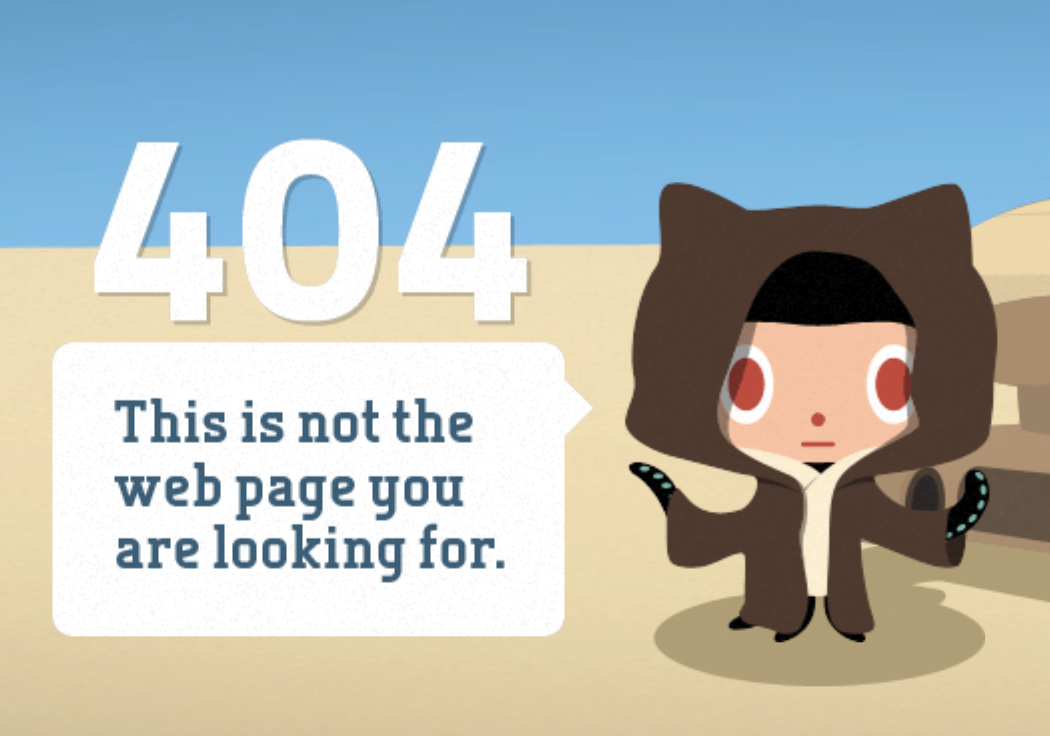
\includegraphics{404.png}
%     \caption[Google's 404 page]{Google's 404 page}
% \end{marginfigure}

% \marginpar{%
%   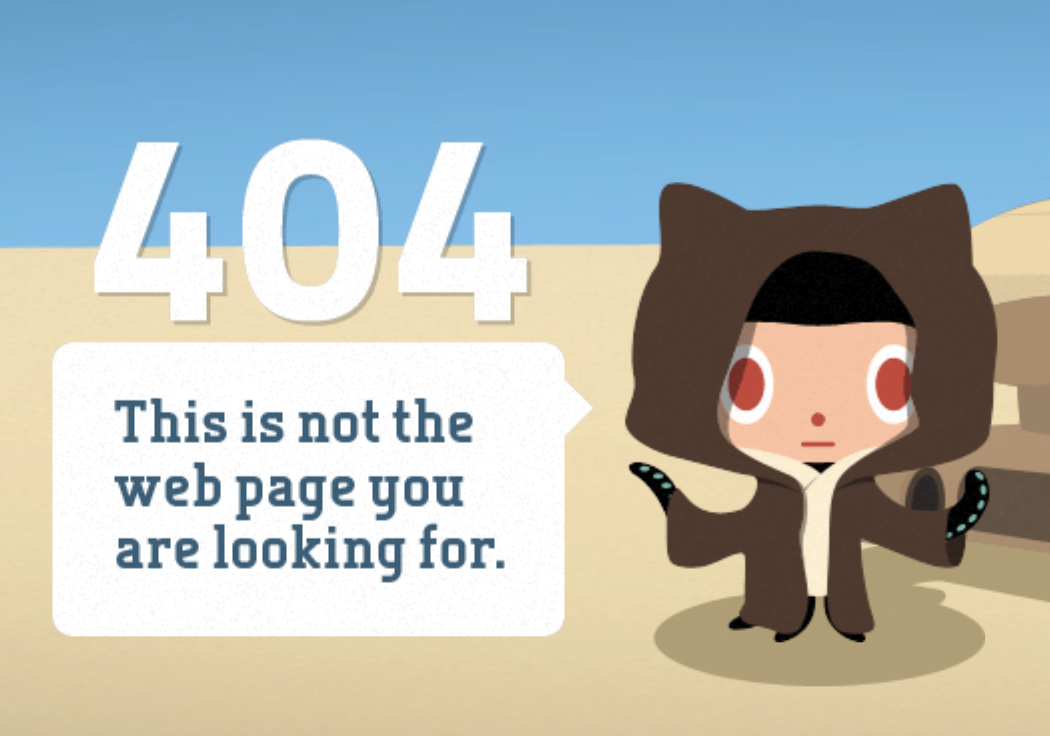
\includegraphics[width=\marginparwidth]{404.png}
%   \captionof{figure}{GitHub's 404 page}
% }
\margingraphic{404.png}{GitHub's 404 page}

You don't have to memorize these, but you'll find that after working with HTTP requests for a while they'll just come naturally. For example, you might be familiar with the infamous code \texttt{404}, which indicates that a resource was not found. You'll come to recognize other codes just like this one.

\begin{kaobox}[title=About the HTML we saw before\dots]
    What was it doing there? It's known as the \kw{body} of the response, and it's being sent back to the client, in essence, because that's what they asked for. Let's break things down. The client sent a \texttt{GET} request, asking the server to send some data back from a particular location (www.example.com). The data that was sent was this HTML code... Do you see where this is going yet? \\ \\
    We know that HTML is used by browsers in order to render web pages, so our client can now successfully render the web page stored on the server. In essence, the client uses this HTTP request in order to receive the data necessary to render a web page! This process happens billions of times per day, and it is the back bone of the whole internet. The internet is built upon servers which store HTML, CSS, and Javascript and your browser uses HTTP requests to request them to be sent to you! Obviously, there's more to the internet than just this, and we could fill many books talking about it, but it's outside the scope of this workshop series. If you're interested take CS 118!
\end{kaobox}

HTML is not the only thing that can be placed in response bodies. In fact, just looking at the \texttt{Accept} section of our HTTP request we can see that images can be as well!

\begin{verbatim}
    Accept: text/html,application/xhtml+xml,application/xml;
    q=0.9,image/avif,image/webp,*/*;q=0.8
\end{verbatim}

Another common data format used in HTTP bodies is known as \kw{JSON}, or Javascript Object Notation. We'll discuss JSON more in detail once we actually see it in action, but for now it suffices to understand that it is a way to encode objects in Javascript as strings. For example, the following code block shows an object called \texttt{heck} and its corresponding JSON string representation:

\vspace{.5cm}

\begin{lstlisting}[language=Java]
    heck = {
        studentOrgRanking: 1,
        color: "#C960FF",
        rizz: 100,
        website: "https://hack.uclaacm.com"
    }

    {
        "studentOrgRanking": 1,
        "color": "#C960FF",
        "rizz": 100,
        "website": "https://hack.uclaacm.com"
    }
\end{lstlisting}

\margingraphic{hack-chad.png}{Rizz 100}

\section{Web API's: What's on the Menu?}

Now that our server and client have a common language, it's time to take things a step further. Let's revisit the restaurant analogy. How does the customer know what they're allowed to order? They can't just demand to be served whatever they want, because the restaurant might not be able to accommodate their request.\sidenote{Yes, there are exceptions, secret menus, etc. But let's be real. If you order off the secret menu, the staff hates you.} That's why every restaurant has a menu! There needs to be a way to let customers know what they can order. Clients and servers are much the same. There needs to be an understanding between them about what the server can do for the client, and this is accomplished using the \kw{API}, or Application Programming Interface. You may have heard this term before. It's another one of those nebulous phrases that gets thrown around a lot, but is rarely defined concretely.

In general, an API is just a way for two computer programs to interact with each other. Think of the customer at a restaurant as one program and the staff as another. The customer hasn't eaten in 16 hours and is craving a burrito with carnitas and guacamole.\sidenote{I am so hungry right now.} Using the menu (the API), the customer is able to enjoy the result of the staff's work and they don't need to attend 4 years of culinary school in order to do it! Put another way, the API allows us to interact with a blackbox and receive meaningful results. API's can be found everywhere in software engineering, but we will be creating more specialized API's called \kw{Web API's}.\sidenote{As the name implies, these are API's that utilize the Web, allowing communication from client to server through HTTP requests.}

\begin{kaobox}[title=Let's take a look at an example of a simple API.]
    
    API's can be expressed in several ways, either using code or English. Let's keep it simple and just use English. Consider a server with the sole purpose being to simulate a cat. The API defines several actions that you, as a pet owner, can take to interact with the cat, and in response the server will send a JSON string (recall that JSON is just a string representation of a Javascript object) with information about the cat and its actions. \\

    The API is defined as follows:
    \begin{verbatim}
    POST FEED: You feed the cat.
    POST WATER: You give the cat a drink.
    POST PET: You pet the cat.
    GET STATUS: You check how the cat is doing.
    POST MEOW: You meow at the cat.
    \end{verbatim}

    These five actions define how you can interact with the cat server. Some of the interactions may have side effects, or an effect on the state of the cat. Also, notice the HTTP method names before each action name! Let's start by petting the cat. Note that the formatting below does not follow HTTP.

    \begin{verbatim}
    REQUEST: POST PET

    RESPONSE: 
    {
        "health": 100,
        "hunger": 10,
        "thirst": 10,
        "action": "Meows and sits down, ready 
                    for more pets."
    }
    \end{verbatim}

    He seems friendly! Let's give him some food.

    \begin{verbatim}
    REQUEST: POST FEED

    RESPONSE: 
    {
        "health": 100,
        "hunger": 50,
        "thirst": 10,
        "action": "Meows gratefully, 
                and attacks the food."
    }
    \end{verbatim}

    Okay, he seems to be enjoying that. Let's pet some more.
    \begin{verbatim}
    REQUEST: POST PET

    RESPONSE: 
    {
        "health": 100,
        "hunger": 50,
        "thirst": 10,
        "action": "Bites your hand. He wasn't 
            done eating yet!"
    }
    \end{verbatim}

    Ouch. How to respond?

    \begin{verbatim}
    REQUEST: POST MEOW

    RESPONSE: 
    {
        "health": 100,
        "hunger": 50,
        "thirst": 10,
        "action": "Looks up from food, confused."
    }
    \end{verbatim}

    Okay, that's enough playing with the cat! Hopefully, this toy example gave you a clearer idea of what an API is as well as its purpose. We'll be creating a real API later in this chapter using Javascript.

\end{kaobox}

Typically, Web API's contain multiple \kw{endpoints}. In general, an endpoint can be thought of as a point of contact between a client and a server. Depending on which endpoint is invoked, the server knows which action to take. In the previous example, we can think of each of the possible five actions as an endpoint. Another common way of thinking about endpoints is as \emph{specific digital locations} of resources located on a server. For example, if we want to access the resource located at \texttt{/MEOW} on a server, we use the \texttt{MEOW} endpoint. You can think about endpoints in whichever way is best for your own mental model, as long as you remember that endpoints are meant to direct the server towards a particular action or resource. And don't worry if things aren't clear yet! We'll be showing concrete examples of all of these concepts in the next few sections.

\margingraphic{kevin.jpg}{This is the cat. His name is Kevin.}

\section{Server Implementations}

As one might expect, there are many ways to go about implementing a server. We know that a server is simply a computer tasked with listening and responding to requests, and clearly this task is not specific to any single programming language. Some popular choices are the following:

\begin{itemize}
    \item Node.js and Express
    \item Python and Django
    \item Python and Flask
    \item C and Pain\sidenote{Pain in the literal sense of the word. Not recommended.}
\end{itemize}

There are countless libraries out there, so no need to reinvent the wheel. Since we're focusing on the MERN stack for Stackschool, we'll be going with Express and Node.\sidenote{Representing the E and N in MERN respectively.} To avoid any confusion let's first discuss what exactly they do, and why they are useful for us when building a server app.

\subsection*{What is Node?}

Originally, Javascript was created as a scripting language for the browser, Netscape, and wasn't intended to be executed outside of that environment.\sidenote{It also took only 10 days for the first version to be developed, which honestly explains a lot.} However, as time has gone on and Javascript has gotten more popular, it has transcended this original functionality. In 2009, a man named Ryan Dahl decided that Javascript would be an excellent language for writing server programs, and created a new runtime environment\sidenote{By runtime environment, I just mean a program that can execute code.} for it outside of the browser. Node was the product of his efforts. Now, years later, it's the most popular non-browser runtime for Javascript and home to a thriving, community driven ecosystem of libraries.\sidenote{We call these libraries packages, and we access them using a program called NPM, or Node Package Manager. Another popular (and, in my opinion, better) package manager is Yarn. We'll be using Yarn for all examples here.} As described on their website, Node is "an asynchronous event-driven JavaScript runtime designed to build scalable network applications." Essentially, it's perfect for servers!

\subsection*{What is Express?}

Node gives you all the fundamentals required to make a server, but why do that if someone's already done most of the work for us? Express is a framework that makes creating server applications far easier by abstracting away most of the HTTP request logic. There are plenty of alternative frameworks, but to stay true to the MERN stack, we'll be going with Express.

\subsection*{Creating Your First Server}

Now that we have all that out of the way, let's get to the fun part. First, make sure you have all the necessary installations. Follow the checklist:

\begin{itemize}
    \item Node. \href{https://nodejs.org/en/download/package-manager/#macos}{Here} is an extensive guide to installing no matter which platform you're on. I recommend using Homebrew if you're on MacOS.\sidenote{Some would recommend using a version manager like NVM, but if you just want to get your hands dirty quickly, the other methods are adequate for now.}
    \item Yarn. This will be your package manager, or the program you use to install node packages (like Express). Once you have Node installed, you can install Yarn by running \texttt{npm install -{}-global yarn} in your shell. 
\end{itemize}

Now in your terminal, navigate to the directory of your choice\sidenote{If you're not familiar with navigating the terminal, check out \href{https://www.digitalocean.com/community/tutorials/basic-linux-navigation-and-file-management}{this} resource.} and run \texttt{yarn init}. This will start the process of creating your server application. It'll prompt you with some basic configuration information, but you can just accept the default values by pressing enter for each one. Don't worry, you can change these values later! After you've completed this step, a new file called \texttt{package.json} should have been generated. This is the configuration file for your server. To install Express, run \texttt{yarn add express}. This should generate a directory called \texttt{node\_modules} and a file called \texttt{yarn.lock}.

Now let's make the server itself. Create a new file called \texttt{server.js}. Within this file, add this boilerplate code:

\begin{lstlisting}[language=Java]
    /**** INIT SERVER ****/
    const express = require('express');
    const app = express();
    app.use(express.json());
    
    /**** DEPLOY SERVER ****/
    const port = 8080;
    
    app.listen(port);
    console.log(`listening on http://localhost:${port}/`);
    console.log("Press Ctrl-C to quit");
\end{lstlisting}

Congrats, you just made your first server! Unfortunately, it doesn't do anything. You can run it with \texttt{node server.js}. Before making it a bit more useful, let's break down what exactly is happening. Take a look at the second line. In Node, the \texttt{require} function is a way to include code from other files within your file.\sidenote{Similar to imports/includes in other languages you may be familiar with. We call the code that we're importing a "module."} In this case, we're including code from the Express package. In the next line, we create an Express app and bind it to a variable. In the final stage of initialization, we tell the app to use something called a \kw{middleware} function. We'll get into these in more detail soon, but for now just know that it's a way to make your life easier. Now, in the deployment section, we define a port, and tell the server to listen on that port. This will affect the URL of your local server.

Alright, now that we've cleared all that up,\sidenote{May be worth a couple more readthroughs if it's still unclear, or get in contact with us on \href{https://discord.gg/xXcJWDUqJj}{Discord}!} its time to add our first endpoint. We'll make an endpoint that requests a random number from the server. It's pretty easy!

\begin{lstlisting}[language=Java,firstnumber=6]
    /**** ROUTES ****/
    app.get("/random", (req, res) => {
        // generate random number from 1-100
        const rand = Math.floor(Math.random() * 100) + 1;

        // send random number in response
        res.send(`${rand}`);
})
\end{lstlisting}

This endpoint can be referred to as \texttt{GET /random}\sidenote{Note that \texttt{/random} is referred to as a \kw{route}. The distinction between endpoints and routes is that endpoints include the HTTP method (i.e. GET, POST, etc.) in their definition. You can have multiple endpoints with the same route, as long as the method is different (so having \texttt{GET /random} and \texttt{POST /random} would be perfectly fine).} and every time it is invoked it will return a string containing a random number from 1-100. You can test it out by starting the server and visiting \url{http://localhost:8080/random} in your browser.\sidenote{In order to start your server, use \texttt{node server.js}.} At a surface level, all that's going on here is that we're using Javascript code to define our server's API. 

\begin{kaobox}[title=Describing the API with English]
    Recall how we defined our API in the cat server example. We can describe our Javascript endpoint definition for random in the same way! 

    \begin{verbatim}
    GET /random: Get a random number from 1-100.
    \end{verbatim}
    
    They're two ways of saying the same thing, except that one of them happens to be real, functional code.
\end{kaobox}

Hopefully, you now have a feel for the general process of creating Express applications. You're now ready to put everything together into a more realistic application.

\section{Demo}

\section{Testing}

\section{Organization}
\setchapterpreamble[u]{\margintoc}

\chapter{Backend Integration}
\epigraph{\emph{"Coming together is the beginning. Keeping together is progress. Working together is success."}}{\- Henry Ford}
 
Now that we're backend experts (more or less), it's time to shift gears. In this chapter we'll be focusing on building the frontend and integrating our backend into it. This will mostly involve a lot of review of frontend topics, although we will be covering several new ideas you've likely never seen before. In particular, how do we make calls to our backend from our frontend? We'll explore this, and more, in the chapter to come.

As mentioned in the Introduction chapter, it will be useful to have some basic background knowledge on several technologies going into this chapter. This includes:

\begin{itemize}
    \item Fundamental Coding Concepts (Think CS31)
    \item Basic Shell Commands (\texttt{cd}, \texttt{ls}, etc.)
    \item HTML/CSS
    \item Javascript
    \item React
\end{itemize}

I recommend checking out our past workshop series, Hackschool, for a refresher on these. Without further ado, let's get started.

\section{The Feed}

It seems most natural to start with the feed for our twitter clone, so let's do that. As good software developers, let's try to brainstorm some things we might need to do before we jump in.\sidenote{And make a plan to address each one.} First of all, we know that all of our posts are stored in our MongoDB database. We can use one of our endpoints to retrieve them!\sidenote{Specifically, \texttt{GET /feed}.} This brings up an important question, however: how can we programmatically make HTTP requests? Recall that in the last chapter we saw there are several ways we can make HTTP requests. As a refresher, here they are again:

\begin{enumerate}
    \item Use a GUI application like Postman
    \item Use a requests library like axios
    \item Use a VSCode extension
\end{enumerate}

It seems that options 1 and 3 are moreso meant for testing rather than any programmatic use, so we're left with one option! Axios is a promise-based\sidenote{That means asynchronous!} HTTP requests library that abstracts away many of the tedious details involved with making HTTP requests. Rather than tell you what it can do, let's just jump in and show an example of a function that utilizes it. Going off of our feed motivation from before, let's write a function that invokes the \texttt{GET /feed} endpoint from our backend and add it to our React app. Make sure you run \texttt{yarn add axios} in your frontend project. To test it out, start your backend in another terminal.

\begin{lstlisting}[language=Java]
    import axios from 'axios';
    const URL = "http://localhost:8080";

    //Gets the entire feed
    function getFeed() {
        axios.get(URL + "/feed")
            .then(response => { 
                console.log(response.data);
            })
            .catch(console.error)
    }
\end{lstlisting}

You should see a log in the console containing your feed! Congratulations, you have officially taken the first true step towards making a full stack application. Recall that axios uses promises, so we must incorporate one of the promise resolution methods we discussed in chapter 2 (in this case \texttt{.then()}). 

If we try calling this function, we see the Array of posts in our MongoDB database in the console. Pretty good! We can now try displaying it on our frontend. 

\subsection*{Mapping}

Before we go any further, let's think about what we want to accomplish here. We want to somehow iterate through each post in our posts array, and display information from each one. Up to this point, the canonical way you have been taught to do this is to use a loop! It might look something like this:

\begin{lstlisting}[language=Java]
    for (let i = 0; i < posts.length; i++>) {
        // display post info for current index
    }
\end{lstlisting}

However, there are a couple problems with this. The biggest among these is that we need to write our code within a JSX return block, which we aren't allowed to do! The \texttt{return} needs a value following it, so we can't just add a for loop after it. To fix this, we use mapping!

Mapping is a way of iterating over an array and performing a set of operations on each item within it. Once we complete iteration, it returns a new array with the operations performed! It can be thought of as a kind of "transformer" function. It transforms the items of an array into a new format using some function and spits out the result. Here's a toy example:

\begin{lstlisting}[language=Java]
    a = ["Nathan", "James", "Nareh", "Christina"]; // array to iterate over

    pog = (name) => { // operation to perform
        return `pog${name}`;
    }

    a.map(pog); // performing pog on each item in a
    // Output: ['pogNathan', 'pogJames', 'pogNareh', 'pogChristina']
\end{lstlisting}

We can also simplify this a bit more by utilizing anonymous functions. Rather than name our operation \texttt{pog}, let's just pass it in directly.\sidenote{We can omit our \texttt{return} keyword here using a special syntactic sugar built into JS! For this to work, we must have a single expression in our function and omit our brackets as well.}

\begin{lstlisting}[language=Java]
    a = ["Nathan", "James", "Nareh", "Christina"]; // array to iterate over

    a.map((name) => }pog${name}\texttt{); // performing pog on each item in a

    // Output: ['pogNathan', 'pogJames', 'pogNareh', 'pogChristina']
\end{lstlisting}

Cool! Let's apply this to our feed. In this case, we want to map every post object in our posts array to a JSX component! Let's do that! Recall that a post contains some content, a user, a like count, and a time stamp indicating when it was posted. \sidenote{You have noticed a warning in the console about adding a "unique key prop." To silence this, simply add \texttt{key={i}} to the \texttt{div} tag.}

\begin{lstlisting}[language=Java]
    return (
        <div>
        {posts.map(post => 
            <div>
            <h3> {post.user} </h3>
            <p> {post.content} - Time: {post.timestamp} - Likes: {post.num_likes}</p>
            </div>        
        )}
        </div>
    );
\end{lstlisting}

Unfortunately, this doesn't seem to be working? What's going on?

\subsection*{React Hooks Recap}

React is lazy. It always strives to do the bare minimum to display the user interface. In particular, it only wants to refresh the UI when there is a visual change to be made. In order to enable this laziness, some smart people designed the \texttt{useState()} hook.\sidenote{Recall that a hook in React is just a function that typically starts with "use" and performs some component related logic (usually).} Using this hook, we can designate a variable to be "watched" for changes. If it changes, then the UI will refresh. Sounds cool right?

In general, \texttt{useState()} looks like this:

\begin{lstlisting}[language=Java]
    const [watchedVar, setWatchedVar] = useState([DEFAULT_VAL]);
\end{lstlisting}

The syntax seems a bit funky, but all thats going on is that useState returns an array of two items: a variable to be watched and a function to set the watched variable. We pass in a default value to the function and we call the setter function when we want to update variables value. Seems a bit convoluted, but trust me when I tell you it more than makes up for it in practice. For a more detailed explanation of \texttt{useState} check out one of our previous \href{https://www.youtube.com/watch?v=ehgl3HpR5xQ}{workshops}!

Consider our feed example. We want our UI to update when we fetch our posts array from our server. We can use \texttt{useState()} as follows:\sidenote{Don't forget to import \texttt{useState}.}

\begin{lstlisting}[language=Java]
    const [posts, setPosts] = useState([]);
\end{lstlisting}

By default, we'll just set posts to be an empty array. In order to set the value of posts, we call the \texttt{setPosts()} function. In fact, let's do this within  \texttt{getFeed()}.

\begin{lstlisting}[language=Java]
    //Gets the entire feed
    function getFeed() {
    axios.get(URL + "/feed")
        .then(response => { 
            setPosts(response.data); // <-- We changed this line
        })
        .catch(console.error)
    }
\end{lstlisting}

As an additional caveat, we only want our API call to be performed when our app is initially loaded.\sidenote{Currently it is being called an obscene amount every time we run our app.} To accomplish this, we use \texttt{useEffect()}! In general, \texttt{useEffect()} looks like the following:

\begin{lstlisting}[language=Java]
    useEffect(() => {
        // perform some task
    }, [dependency1, dependency2, ...])
\end{lstlisting}

The function passed to the \texttt{useEffect()} hook will be called whenever one of the dependencies in the dependency array is updated! If the array is empty, it will only be called upon initial app load. Again, check out the \href{https://www.youtube.com/watch?v=ehgl3HpR5xQ}{workshop} we linked before for more information on this, but here's how we use it in our demo app:\sidenote{Note that, just like \texttt{useState}, \texttt{useEffect} needs to be imported from react.}

\begin{lstlisting}[language=Java]
    useEffect(() => {
        getFeed();
    }, []);
\end{lstlisting}

We know have our feed! Granted, it looks quite ugly, but let's take this W for now. 

\section{Profiles and Navigation}

\section{Finishing Touches}

% \chapter{Advanced Frontend}

\blindtext


% \appendix % From here onwards, chapters are numbered with letters, as is the appendix convention

% \pagelayout{wide} % No margins
% \addpart{Appendix}
% \pagelayout{margin} % Restore margins

% \chapter{Some more blindtext}

% \blindtext

%----------------------------------------------------------------------------------------

\backmatter % Denotes the end of the main document content
\setchapterstyle{plain} % Output plain chapters from this point onwards

%----------------------------------------------------------------------------------------
%	BIBLIOGRAPHY
%----------------------------------------------------------------------------------------

% The bibliography needs to be compiled with biber using your LaTeX editor, or on the command line with 'biber main' from the template directory

% \defbibnote{bibnote}{Here are the references in citation order.\par\bigskip} % Prepend this text to the bibliography
% \printbibliography[heading=bibintoc, title=Bibliography, prenote=bibnote] % Add the bibliography heading to the ToC, set the title of the bibliography and output the bibliography note

%----------------------------------------------------------------------------------------
%	INDEX
%----------------------------------------------------------------------------------------

% The index needs to be compiled on the command line with 'makeindex main' from the template directory

% \printindex % Output the index

\end{document}
